\documentclass[a4paper,12pt]{article}
\usepackage[utf8]{inputenc} % encodage du fichier
\usepackage[french]{babel} % document en francais
\usepackage[T1]{fontenc} % pour les caracteres accentues
\usepackage[french]{algorithm2e}
\usepackage{pseudocode}
\usepackage{graphicx}
\usepackage{geometry}

\geometry{top=2cm, bottom=2cm, left=2cm, right=2cm}      

\setlength{\oddsidemargin}{-5pt} % Marge gauche sur pages impaires
\setlength{\textwidth}{481pt} % Largeur de la zone de texte (17cm)
\setlength{\headheight}{13pt} % Haut de page
\setlength{\headsep}{20pt} % Entre le haut de page et le texte


\begin{document}

\pagestyle{empty}

\begin{flushright}
    
\includegraphics[width=3cm]{figures/logo_insa.png} % Remplacez 'logo.png' par le chemin vers votre fichier de logo
\end{flushright}

% Titre principal
\vspace{5cm} 
\begin{center}
    {\huge \textbf{PI Conception d'un Robot Intelligent}} \\[0.5cm]
    {\large DIOP Amsatou EL OMARI BOUYA Lina GUÉNOT Tom LEVASSEUR Nathan VESPIER Michel} \\[0.3cm]
    {\large 6 janvier 2025}
\end{center}

\vspace{1cm} 
\begin{center}
    {\textbf{Objectif}} \\[0.5cm]
    {Concevoir et construire un robot suiveur de ligne capable de sortir d'un labyrinthe le plus vite possible}\\
    \vspace{2cm} 
    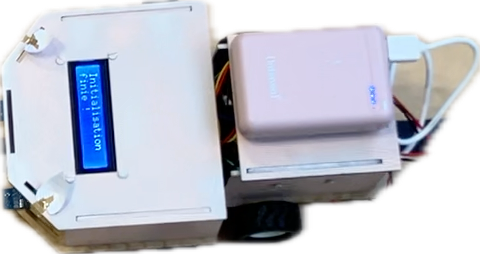
\includegraphics[width = 10cm]{figures/image_Robot.png}
\end{center}

\newpage
\pagestyle{plain}
\setcounter{page}{1}
\tableofcontents

\newpage
% Début du document principal
\section*{Introduction}

\section{Informatique}
\subsection{Analyse}
\subsection{Conception préliminaire}
\subsection{Conception détaillée}
\subsection{Tests}
\subsection{Problèmes recontrés}

\newpage
\section{Électronique}
\subsection{Description des composants}

Nous avons séparé le câblage en trois pôles:
\begin{itemize}
    \item Un pôle Son
    \item Un pôle Vision
    \item Un pôle Moteur
\end{itemize}

\noindent Des $wagos$ sont utilisés pour centraliser le GROUND et les alimentations de la RaspBerry lorsque c'est nécessaire.\\

\large Pôle Son \\
Le premier pôle comprend le système émetteur-récepteur d'ultrasons et le buzzer.
Placé à l'avant, le rôle de ce premier est de calculer la distance qui sépare l'avant du Robot d'un potentiel obstacle.
Si cette distance descend en dessous d'un seuil défini, le Robot doit s'arrêter.
Le buzzer est quand à lui utilisé pour émettre un signal sonore, notament si le Robot s'arrête lorsqu'il rencontre un obstacle.\\

\large Pôle Vision \\
Le deuxième pôle se compose de l'écran LCD, qui est placé sur le dessus du Robot et des trois capteurs de ligne.
Le rôle de l'écran LCD est d'afficher des informations.
Dans le cadre de notre projet, nous l'utilisons pour indiquer les différents ordres que le Robot doit suivre, ainsi que son état d'évolution dans le labyrinthe (lorsqu'il est sorti par exemple).
Nous l'avons également utilisé pour localiser des erreurs lors de nos tests.

Ensuite, les capteurs de ligne sont faits pour envoyer un signal en fonction de la luminosité qu'ils détectent.
C'est le contraste entre les lignes et le reste des tuiles qui les rendent intéressants dans la détection de ligne (comme leur nom l'indique).
Grâce à ces capteurs, nous pouvons détecter les situations dans lesquelles se trouvent le Robot afin qu'il réagisse en conséquence.\\

% Disposition des capteurs (avant = + de marge sur le temps de réaction)
% Quelles combinaisons utiliser pour se repérer 
% Avantage : grande vitesse de réaction, cf video, robot tres efficace
% inconvenient : 1 cas ou le robot bug c'est lorsqu'il se redresse vers une intersection

\large Pôle Moteur \\
Le dernier pôle est bien évidemment dédié aux moteurs.
Ces derniers sont placés à l'arrière du Robot, car c'était à cet emplacement que cela nous paraissait le plus stable, avec une roue ronde à l'avant.
La carte L293D est vissée aux parois du châssis afin de faciliter son accès pour les interventions que nous avons dû faire dessus.

\begin{table}[!h]
    \begin{center}
        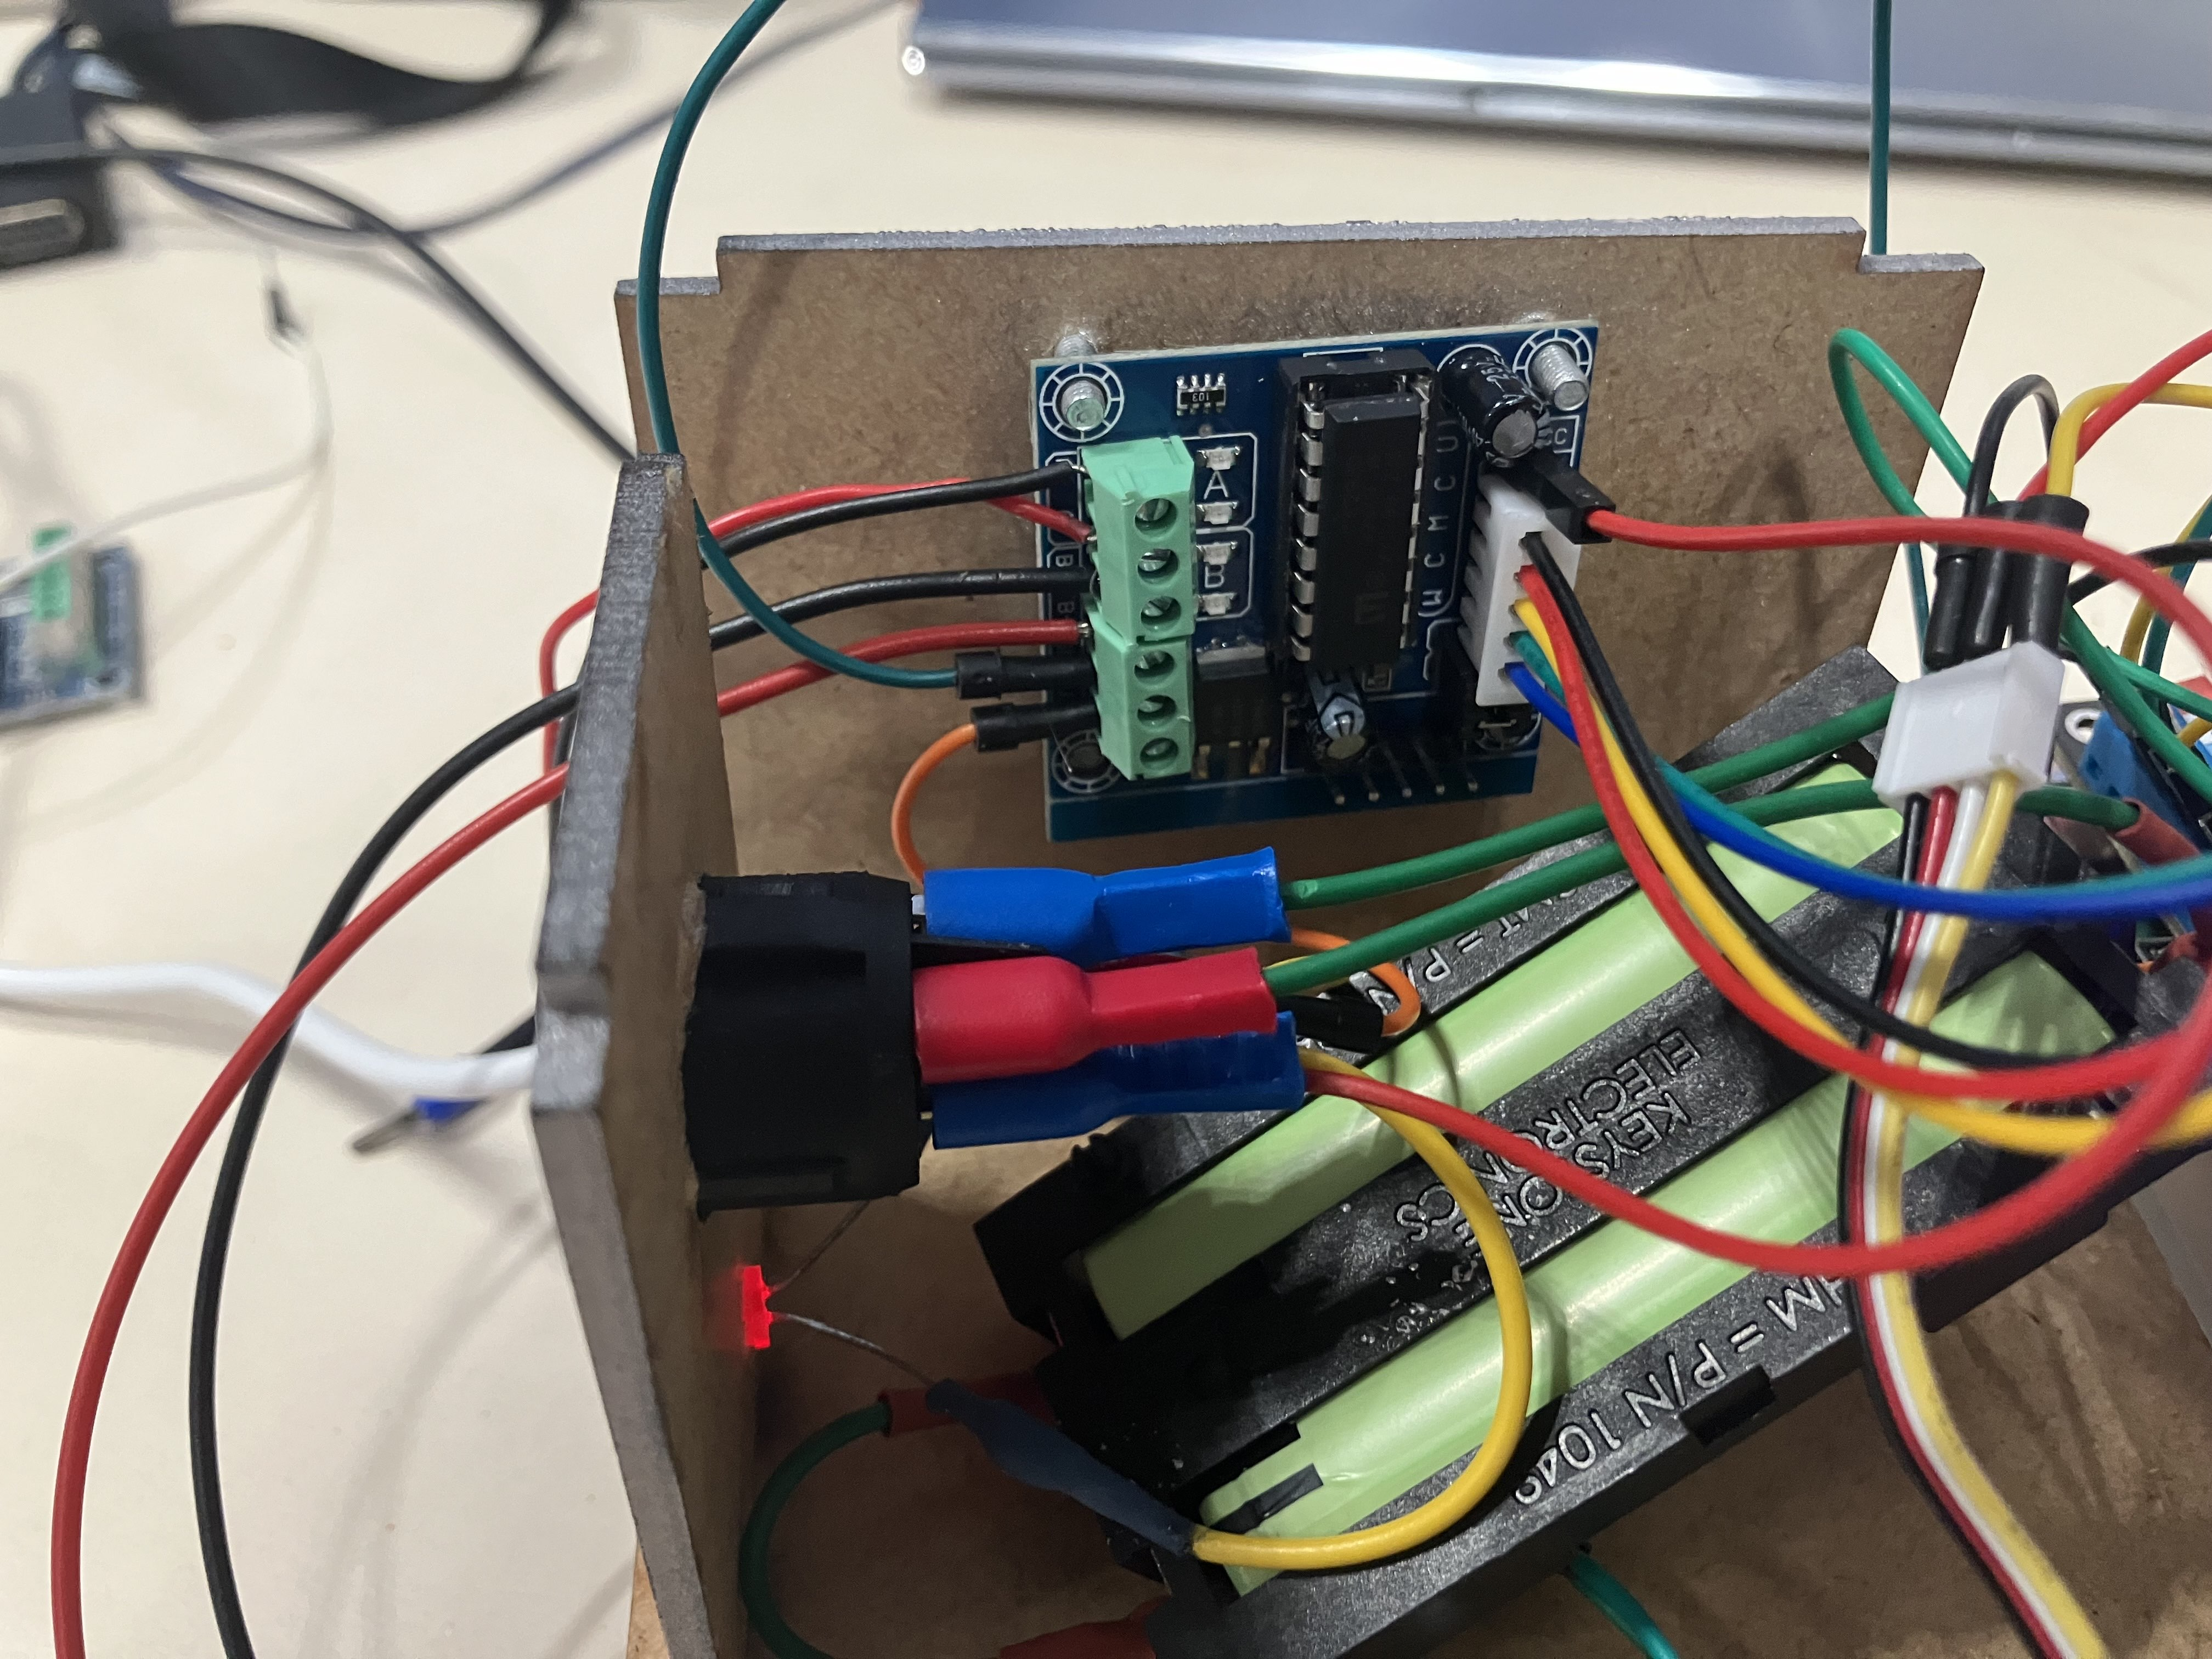
\includegraphics[width = 10cm]{figures/moteursRobot.jpg}
    \end{center}
    \caption{Emplacement des moteurs}
\end{table}

% On nous a demandé de mettre un interrupteur et une LED = protection = resistance
% Pour pas baisser la tension delivrer a la carte et aux moteurs => montage en série
% soudure au niveau du boitier à pile et "pince" pour l'interrupteur


\begin{table}[!h]
    \begin{center}
        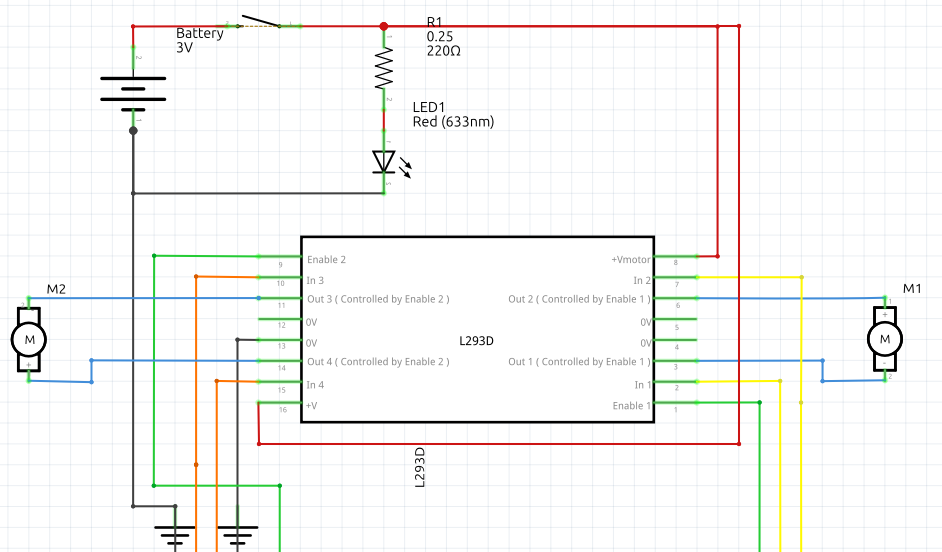
\includegraphics[width = 15cm]{figures/schemaElecMoteurs.png}
        \caption{Schéma électrique du pôle Moteur}     
    \end{center}
\end{table}


\subsection{Schéma électrique}

Le schéma électrique a été fait sur \textit{Fritzing} au début du projet.

Au niveau du choix des branchements, nous avons le plus possible essayé de rapprocher les numéros des GPIO lorsqu'ils étaient utilisés par le même composant, ou un composant similaire.
Par exemple, les pins IN1 et IN2 du moteur 1 sont branchées sur les GPIO 20 et 21 tandis que les capteurs positionnés à droite et à gauche sont branchés sur les GPIO 7 et 8.\\
Cependant, nous avons tout de même privilégié un branchement tel que le schéma électrique numérique soit le plus lisible possible tant que cela était possible.
Cela permet une meilleure compréhension générale du câblage, et rend la résolution de problèmes plus efficace.

Lorsque nous avons monté le Robot, nous avons d'abord fait tous les branchements nécessaires avant de percer le châssis et de le fermer.
Ainsi, l'entièreté de nos câbles ont pu rentrer dans le Robot (à part ceux reliés aux moteurs) et les interventions sur les branchements était facilitées.

\begin{table}[!h]
    \begin{center}
        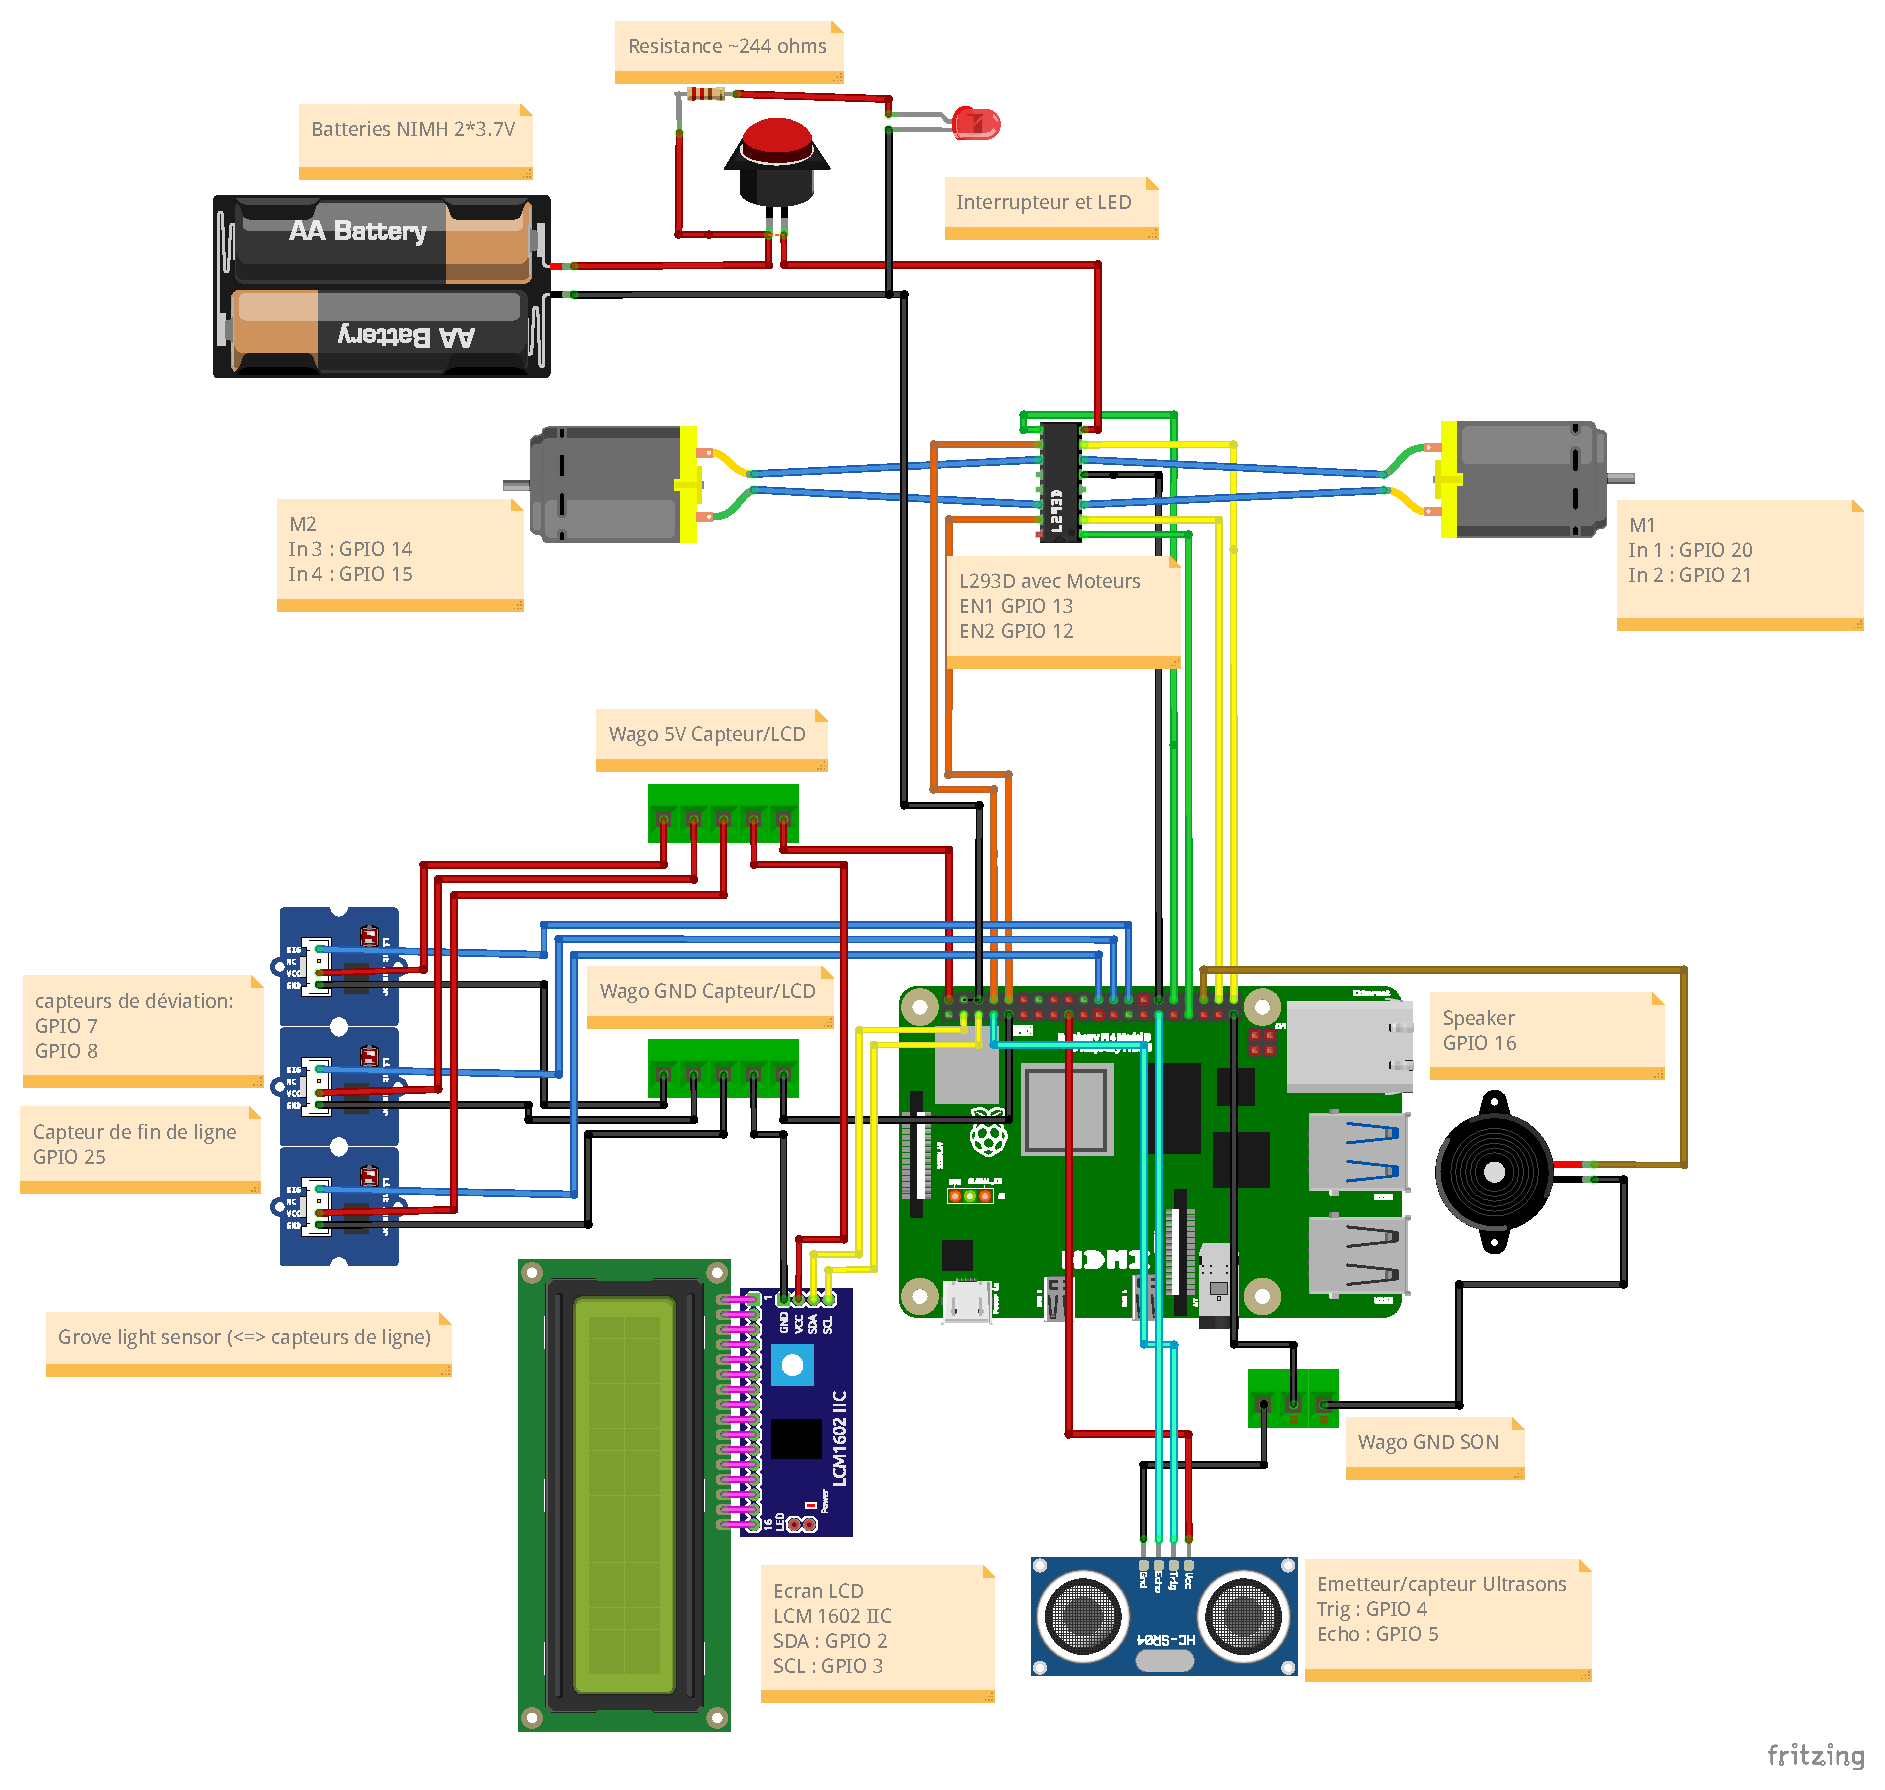
\includegraphics[width = 16cm]{figures/ElectricScheme_PISmartRobot.pdf}
    \end{center}
    \caption{Schéma électrique}
\end{table}
\newpage


\subsection{Algorithme de déplacement}

% -----------------------------PSEUDO CODE----------------------------------------------
\noindent\textbf{procedure} ROBOT\_evolutionRobot ()

\begin{tabular}{ll}
    \textbf{Déclaration:} & prochaineAction: \textbf{Chaine de caractères}\\
     & etat: \textbf{ROBOT\_EtatDAvancement}\\
\end{tabular}

\noindent\textbf{début}

    \begin{algorithm}[H]
        etat $\leftarrow$ Avancer\\
        \Tq{prochaineAction $\neq$ FIN}{
            \textbf{lire} (prochaineAction)\\
            \Suivant{etat}{
                \Cas{Avancer}{ROBOT\_avancer (etat)}
                \Cas{Intersection}{ROBOT\_intersection (etat, prochaineAction)}
                \Cas{Urgence}{ROBOT\_urgence ()}
                }
        }
    \end{algorithm}

    \noindent\textbf{fin}
% -----------------------------PSEUDO CODE----------------------------------------------
\begin{center}
    \textit{Algorithme de ROBOT\_evolutionRobot}
\end{center}

Pour élaborer l'algorithme de déplacement du robot nous avons considéré qu'il pouvait se retrouver dans 4 états différents:
\begin{itemize}
    \item En avancée
    \item Sur une intersection
    \item En situation d'urgence
    \item Sorti du labyrinthe
\end{itemize} 

Nous avons donc une variable $etat$ du type \textbf{ROBOT\_EtatDAvancement} qui est mise à jour à chaque tour d'une boucle qui ne s'arrête que lorsque la suite d'ordre que nous lui fournissons s'achève.
Selon la valeur de cette variable $etat$, différentes fonctions sont appelées afin de faire évoluer le Robot.

La première est la fonction ROBOT\_avancer, qui met les moteurs en marche avant et qui adapte la trajectoire du robot grâce aux capteurs.

Ensuite, la fonction ROBOT\_intersection agit selon l'ordre lu par l'algorithme principal. Elle fait tourner le Robot à droite ou à gauche ou bien le fait continuer tout droit.
Le Robot effectue un virage sur place, nous avons donc paramétré un temps d'attente afin de positionner correctement le centre de rotation du robot sur l'intersection.

La fonction, ROBOT\_urgence, est la fonction qui est appelée lorsqu'un obstacle est détecté. Son rôle est d'arrêter les moteurs et d'allumer le buzzer.

\subsection{Problèmes recontrés}

La première difficulté que nous pouvons citer porte sur l'émetteur-récepteur d'ultrasons.
Malheureusement, l'algorithme utilisé ne parvenait pas à sortir d'une boucle infinie ce qui rendait le Robot incapable de suivre les autres programmes.
Nous avons tenté de paralléliser ce dispositif mais sans succès, c'est pourquoi nous n'avons pas pu présenter cette option lors de la soutenance.\\

Pendant une grande partie du projet, nous avions le sentiment d'avoir une longueur de retard sur les autres groupes à propos de la partie électronique. 
Ce retard était dû aux nombreuses discussions que nous avions eu en amont sur la conception du Robot.
Nous avons discuté du nombre de capteurs, de la position des moteurs et d'autres dispositifs pendant plusieurs séances avant de commencer à percer et à souder.
Au final, cela ne nous a pas desservi; effectivement, après le montage, tous le câblage rentrait parfaitement dans le châssis et la plupart des composants ont fonctionné du premier coup.
De plus, la plupart des erreurs rencontrées venaient des codes utilisés.

Cependant, lors de nos premiers esssais, les moteurs ne répondaient pas. C'était une simple erreur de câblage sans gravité (aucun matériel n'a été dégradé), 
mais avec la fatigue, nous avons mal vérifié l'ensemble des connectiques et le problème ne fût résolu que lors de la séance d'essais suivante.

Avec ce retard accumulé, nous avons manqué de temps pour les derniers réglages, c'est pourquoi un dernier bug subsistait lors de la présentation du Robot.\\

\section{Voies d'amélioration}

Notre Robot possède de nombreux inconvénients.
Tout d'abord, le programme de recherche du plus court chemin n'est pas terminé, ce qui constitue un gros désavantage.
Ensuite, notre choix de représentation du Labyrinthe en C convient pour cette application simple et cadrée, mais elle n'est pas très portable.
Une représentation plus complexe comme les graphes aurait surement été préférable pour faciliter son utilisation. 

Ensuite, le système de redressement n'est pas au point car il gêne la détection d'intersection. De plus, la détection de sa condition d'arrêt laisse à désirer.
Nous aurions pu utiliser des capteurs supplémentaires afin de séparer la détection d'intersection du redressement ou alors rechercher un algorithme plus complexe servant à remettre le Robot dans une position correcte à chaque grosse déviation.
De plus, comme mentionné précédemment, le système de détection d'obstacle ne fonctionne pas du tout.

Une autre voie d'amélioration possible porte sur notre méthode de travail.
Afin de rendre la résolution de problème plus efficace, il aurait fallu définir en amont un protocole à suivre qui aiderait à revoir l'ensemble des éléments à l'origine d'un potentiel problème rencontré.
Avec une telle méthode, nous aurions peut-être perdu moins de temps à chercher où étaient nos erreurs, surtout que la plupart du temps, elles sont très facilement corrigées.

Cette remarque vaut notamment pour la partie électronique et le montage du Robot, pour la partie algorithmie, il faudrait coder un ensemble de tests avant de dévelloper nos programmes (comme le suggère le cycle en V).

\section*{Conclusion}
\section{Répartition des tâches}
\end{document}